\documentclass{article}%
\usepackage[T1]{fontenc}%
\usepackage[utf8]{inputenc}%
\usepackage{lmodern}%
\usepackage{textcomp}%
\usepackage{lastpage}%
\usepackage{geometry}%
\geometry{margin=1in,headheight=14pt,headsep=25pt}%
\usepackage{hyperref}%
\usepackage{enumitem}%
\usepackage{fancyhdr}%
\usepackage{xcolor}%
\usepackage{url}%
\usepackage{breakurl}%
\usepackage{amsmath}%
\usepackage{amssymb}%
\usepackage{mathtools}%
\usepackage{amsthm}%
\usepackage{thmtools}%
\usepackage{float}%
\usepackage{subcaption}%
\usepackage[font=small,labelfont=bf]{caption}%
%

            \hypersetup{
                colorlinks=true,
                linkcolor=blue,
                filecolor=magenta,
                urlcolor=blue,
                breaklinks=true,
                bookmarks=true,
                pdfborder={0 0 0}
            }
            \urlstyle{same}
            \Urlmuskip=0mu plus 1mu  % URL breaking in nicer spots

            % Math configuration
            \everymath{\displaystyle}
            \setlength{\jot}{10pt}  % Increase spacing between equations

            \pagestyle{fancy}
            \fancyhf{}
            \rhead{Generated on \today}
            \cfoot{\thepage}

            % Better Unicode support
            \usepackage[utf8]{inputenc}
            \usepackage{newunicodechar}
            \setlength{\itemsep}{1em} % Adds spacing between items

            % Configure itemize settings globally
            \setlist[itemize]{nosep}
            \setlist[itemize]{leftmargin=*}

            % Remove section numbering
            \renewcommand{\thesection}{}
            \renewcommand{\thesubsection}{}

            % Adjust caption spacing around figures
            \setlength{\abovecaptionskip}{0pt}
            \setlength{\belowcaptionskip}{5pt}
        %
\lhead{Lecture: 2024{-}09{-}19{-}DualityExamples}%
\title{2024{-}09{-}19{-}DualityExamples}%
\author{Generated by Scribe.AI}%
\date{\today}%
%
\begin{document}%
\normalsize%
\maketitle%
\section{Slide 1}%
\label{sec:Slide1}%
\subsection{Content}%

\textbf{Duality - Interpretations} \\
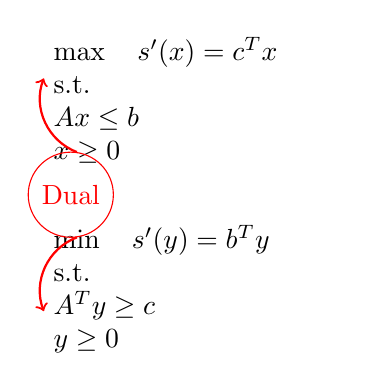
\begin{tikzpicture}[scale=0.8]
\node (primal) at (0,0) {
\begin{minipage}{0.3\textwidth}
$\max \quad s'(x) = c^Tx$ \\
s.t. \\
$Ax \le b$ \\
$x \ge 0$
\end{minipage}
};
\node (dual) at (0,-3) {
\begin{minipage}{0.3\textwidth}
$\min \quad s'(y) = b^Ty$ \\
s.t. \\
$A^Ty \ge c$ \\
$y \ge 0$
\end{minipage}
};
\node[circle,draw,red] (dual_label) at (-2,-1.5) {Dual};
\draw[->,red,thick,bend left=45] (dual_label) to (primal);
\draw[->,red,thick,bend right=45] (dual_label) to (dual);
\end{tikzpicture}
%
\subsection{Description}%
Slide 1 of 8 in a Linear Programming course introduces the concept of duality.  The slide presents a primal linear programming problem in the form:
$\max \quad s'(x) = c^Tx$
s.t.
$Ax \le b$
$x \ge 0$
and its corresponding dual linear programming problem:
$\min \quad s'(y) = b^Ty$
s.t.
$A^Ty \ge c$
$y \ge 0$
A red circle labeled "Dual" connects the two problems with curved arrows, visually representing the duality relationship.  The notation $c^T$, $b^T$, and $A^T$ represent the transpose of vectors $c$ and $b$, and matrix $A$, respectively. The context of the course makes it clear that this slide is setting the stage for a discussion of duality theory in linear programming, which is a fundamental concept in optimization.%
\subsection{Figures}%
\begin{figure}[H]%
\centering%
\begin{subfigure}[b]{0.15\textwidth}%
\centering%

\includegraphics[width=\textwidth]{/Users/ashoksaravanan/Coding/ScribeLec/server/output/MA 421/lectures/2024-09-19-DualityExamples/figures/1.1.png}%
\caption{A diagram showing the primal and dual linear programming problems.  The primal problem is a maximization problem, and the dual problem is a minimization problem.  There is a red circle labeled "Dual" with red arrows indicating the relationship between the primal and dual problems.}%
\end{subfigure}%
\end{figure}

%
\newpage%
\section{Slide 2}%
\label{sec:Slide2}%
\subsection{Content}%

\textbf{Diet Problem} \\
$m$ \quad Nutrients (eg. Vitamins) \quad $N_i$ : $i = 1, 2, \dots, m$ \\
$n$ \quad Foods \quad $F_j$ : $j = 1, 2, \dots, n$ \\
$a_{ij} = $ amount of $N_i$ in 1 unit of $F_j$ \\
$b_i = $ minimum (monthly) intake of $N_i$ \\
$c_j = $ price (cost) of $F_j$ \\
$\boxed{x_j = \text{amount of consumption of } F_j}$
%
\subsection{Description}%
Slide 2 of 8 in a Linear Programming course introduces the "Diet Problem."  The slide defines the parameters of the problem:  $m$ represents the number of nutrients ($N_i$), $n$ represents the number of foods ($F_j$), $a_{ij}$ represents the amount of nutrient $i$ in one unit of food $j$, $b_i$ represents the minimum monthly intake required for nutrient $i$, and $c_j$ represents the price (or cost) of food $j$.  Crucially, the slide defines $x_j$ as the decision variable, representing the amount of food $j$ to be consumed, which is highlighted by a red box.  This sets the stage for formulating the diet problem as a linear programming optimization problem in subsequent slides. The notation clearly indicates that this is a linear programming problem with $m$ constraints (one for each nutrient) and $n$ variables (one for each food).%
\subsection{Figures}%
\begin{figure}[H]%
\centering%
\begin{subfigure}[b]{0.15\textwidth}%
\centering%

\includegraphics[width=\textwidth]{/Users/ashoksaravanan/Coding/ScribeLec/server/output/MA 421/lectures/2024-09-19-DualityExamples/figures/2.1.png}%
\caption{A handwritten slide defining the parameters of a diet problem. The box around $x_j$ highlights its importance as the decision variable.}%
\end{subfigure}%
\end{figure}

%
\newpage%
\section{Slide 3}%
\label{sec:Slide3}%
\subsection{Content}%

\textbf{Diet Problem} \\
\begin{tabular}{|c|c|c|c|c|c|c|}
\hline
$N_i \backslash F_j$ & $C_1$ & $C_2$ & $C_3$ & $C_j$ & $\cdots$ & $C_n$ \\
\hline
$b_1$ & 1 &  &  &  &  &  \\
\hline
$b_2$ & 2 &  &  &  &  &  \\
\hline
$b_i$ & $i$ &  &  & $a_{ij}$ &  &  \\
\hline
$\vdots$ & $\vdots$ &  &  &  &  &  \\
\hline
$b_m$ & $m$ &  &  &  &  &  \\
\hline
\end{tabular}
%
\subsection{Description}%
Slide 3 of 8 in a Linear Programming course presents a tabular representation of the diet problem introduced in the previous slide. The table visually organizes the parameters of the problem. Rows represent nutrients ($N_i$, $i = 1, \dots, m$), and columns represent foods ($F_j$, $j = 1, \dots, n$).  The entry $a_{ij}$ in the table represents the amount of nutrient $i$ present in one unit of food $j$. The first column lists the minimum required daily intake ($b_i$) for each nutrient $i$. The top row shows the cost ($C_j$) of each food $j$.  This tabular representation provides a clear and concise way to visualize the data and relationships between nutrients and foods, setting the stage for formulating the linear programming model in the following slides. The use of a table is a common way to represent the constraints and objective function in linear programming problems.%
\subsection{Figures}%
\begin{figure}[H]%
\centering%
\begin{subfigure}[b]{0.15\textwidth}%
\centering%

\includegraphics[width=\textwidth]{/Users/ashoksaravanan/Coding/ScribeLec/server/output/MA 421/lectures/2024-09-19-DualityExamples/figures/3.1.png}%
\caption{A table representing the diet problem. The rows represent nutrients ($N_i$), and the columns represent foods ($F_j$). The entry $a_{ij}$ represents the amount of nutrient $i$ in food $j$. The first column shows the minimum required intake ($b_i$) for each nutrient. The top row shows the cost ($C_j$) of each food.}%
\end{subfigure}%
\end{figure}

%
\newpage%
\section{Slide 4}%
\label{sec:Slide4}%
\subsection{Content}%

\textbf{Diet Problem} \\
\begin{tabular}{|c|c|c|c|c|c|c|}
\hline
$N_i \backslash F_j$ & $C_1$ & $C_2$ & $C_3$ & $C_j$ & $\cdots$ & $C_n$ \\
\hline
$b_1$ & 1 &  &  &  &  &  \\
\hline
$b_2$ & 2 &  &  &  &  &  \\
\hline
$b_i$ & $i$ &  &  & $a_{ij}$ &  &  \\
\hline
$\vdots$ & $\vdots$ &  &  &  &  &  \\
\hline
$b_m$ & $m$ &  &  &  &  &  \\
\hline
\end{tabular}
%
\subsection{Description}%
Slide 4 of 8 in a Linear Programming course continues the presentation of the diet problem.  This slide provides a tabular representation of the problem's data. The table has rows representing nutrients ($N_i$, where $i = 1, \dots, m$) and columns representing foods ($F_j$, where $j = 1, \dots, n$).  The cell at the intersection of row $i$ and column $j$ contains the value $a_{ij}$, representing the amount of nutrient $i$ in one unit of food $j$. The first column shows the minimum required daily intake ($b_i$) for each nutrient $i$. The top row indicates the cost ($C_j$) of each food $j$.  This tabular format visually organizes the data, making it easier to understand the relationships between nutrients and foods before formulating the linear programming model in subsequent slides.  The handwritten nature of the table suggests this is a lecture slide, not a formal document. The highlighted cell containing $a_{ij}$ emphasizes its importance in the problem's constraints.%
\subsection{Figures}%
\begin{figure}[H]%
\centering%
\begin{subfigure}[b]{0.15\textwidth}%
\centering%

\includegraphics[width=\textwidth]{/Users/ashoksaravanan/Coding/ScribeLec/server/output/MA 421/lectures/2024-09-19-DualityExamples/figures/4.1.png}%
\caption{A table representing the diet problem. The rows represent nutrients ($N_i$), and the columns represent foods ($F_j$). The entry $a_{ij}$ represents the amount of nutrient $i$ in food $j$. The first column shows the minimum required intake ($b_i$) for each nutrient. The top row shows the cost ($C_j$) of each food.}%
\end{subfigure}%
\end{figure}

%
\newpage%
\section{Slide 5}%
\label{sec:Slide5}%
\subsection{Content}%

\textbf{Diet Problem} \\
\text{minimize cost:} \quad f(x) = \sum_j c_j x_j \\
s.t. \\
\sum_j a_{ij} x_j \ge b_i \\
x_j \ge 0
%
\subsection{Description}%
Slide 5 of 8 in a Linear Programming course presents the mathematical formulation of the Diet Problem. The slide states the objective function as minimizing the total cost,  $f(x) = \sum_j c_j x_j$, where $c_j$ is the cost of food $j$ and $x_j$ is the amount of food $j$ consumed.  The constraints are given as $\sum_j a_{ij} x_j \ge b_i$, ensuring that the minimum required intake ($b_i$) of nutrient $i$ is met, where $a_{ij}$ represents the amount of nutrient $i$ in food $j$.  The non-negativity constraint $x_j \ge 0$ is also included.  Handwritten annotations clarify the meaning of the variables and parameters, with arrows pointing to the relevant terms.  The terms "cost of $c_j$", "consumption of $f_j$", and "min. intake of $N_i$" are highlighted in red to emphasize their importance. The slide builds upon the previous slides by translating the verbal description and tabular representation of the Diet Problem into a formal mathematical optimization problem.%
\subsection{Figures}%
\begin{figure}[H]%
\centering%
\begin{subfigure}[b]{0.15\textwidth}%
\centering%

\includegraphics[width=\textwidth]{/Users/ashoksaravanan/Coding/ScribeLec/server/output/MA 421/lectures/2024-09-19-DualityExamples/figures/5.1.png}%
\caption{Handwritten notes describing the Diet Problem in linear programming. The objective function is to minimize the cost, represented by $f(x) = \sum_j c_j x_j$. The constraints are $\sum_j a_{ij} x_j \ge b_i$ and $x_j \ge 0$.  Arrows point to the terms and explain their meaning.  The text "cost of $c_j$" and "consumption of $f_j$" are written in red, and "min. intake of $N_i$" is also written in red.}%
\end{subfigure}%
\end{figure}

%
\newpage%
\section{Slide 6}%
\label{sec:Slide6}%
\subsection{Content}%

\textbf{Diet Problem} \\
\begin{tabular}{|c|c|c|c|c|c|c|}
\hline
$N_i \backslash F_j$ & $C_1$ & $C_2$ & $C_3$ & $C_j$ & $\cdots$ & $C_n$ \\
\hline
$b_1$ & 1 &  &  &  &  &  \\
\hline
$b_2$ & 2 &  &  &  &  &  \\
\hline
$b_i$ & $i$ &  &  & $a_{ij}$ &  &  \\
\hline
$\vdots$ & $\vdots$ &  &  &  &  &  \\
\hline
$b_m$ & $m$ &  &  &  &  &  \\
\hline
\end{tabular}
%
\subsection{Description}%
Slide 6 of 8 in a Linear Programming course shows a table summarizing the data for the diet problem.  The table's rows represent nutrients ($N_i$, $i = 1, \dots, m$), and columns represent foods ($F_j$, $j = 1, \dots, n$).  The entry $a_{ij}$ denotes the amount of nutrient $i$ in one unit of food $j$. The first column lists the minimum required daily intake ($b_i$) for each nutrient. The top row shows the cost ($C_j$) for each food $j$.  A light orange rectangle highlights the first three columns of the table, possibly to emphasize these foods in a subsequent discussion or example. This slide visually reinforces the data structure introduced in previous slides, preparing the students for the next steps in formulating and solving the linear programming model. The handwritten style suggests this is a lecture slide, not a formal document.%
\subsection{Figures}%
\begin{figure}[H]%
\centering%
\begin{subfigure}[b]{0.15\textwidth}%
\centering%

\includegraphics[width=\textwidth]{/Users/ashoksaravanan/Coding/ScribeLec/server/output/MA 421/lectures/2024-09-19-DualityExamples/figures/6.1.png}%
\caption{A table representing the diet problem. The rows represent nutrients ($N_i$), and the columns represent foods ($F_j$). The entry $a_{ij}$ represents the amount of nutrient $i$ in food $j$. The first column shows the minimum required intake ($b_i$) for each nutrient. The top row shows the cost ($C_j$) of each food.  A light orange rectangle highlights the cells corresponding to foods $C_1$, $C_2$, and $C_3$.}%
\end{subfigure}%
\end{figure}

%
\newpage%
\section{Slide 7}%
\label{sec:Slide7}%
\subsection{Content}%

\textbf{Diet Problem} \\
\underline{\text{Replacement of food by pills for each } N_i \text{'s}} \\
N_i = \text{pills} \quad i = 1, 2, \dots, m \\
\boxed{Y_i = \text{unit price of pill for } N_i} \\
1 \text{ unit of } F_j \text{ contains } a_{ij} \text{ unit of } N_i \\
\text{Price/Value of (1 unit) } F_j = \sum_i Y_i a_{ij} \\
\underline{\text{Maximize profit by selling pills}}
%
\subsection{Description}%
Slide 7 of 8 in a Linear Programming course introduces a variation of the Diet Problem. Instead of minimizing cost, this slide focuses on maximizing profit by replacing food with pills.  The handwritten notes define $N_i$ as pills for nutrient $i$, where $i$ ranges from 1 to $m$.  $Y_i$ represents the unit price of pill $i$.  The amount of nutrient $i$ in one unit of food $j$ is denoted by $a_{ij}$, which is consistent with the notation used in previous slides. The price or value of one unit of food $j$ is calculated as $\sum_i Y_i a_{ij}$. The objective is to maximize profit by selling these pills, representing a dual problem to the original minimization problem.  The underlining highlights the problem's title and objective. The boxed equation for $Y_i$ emphasizes its importance as a key variable in the new formulation. The context of the course is crucial for understanding this as a reformulation of the diet problem, introducing the concept of duality in linear programming.%
\subsection{Figures}%
\begin{figure}[H]%
\centering%
\begin{subfigure}[b]{0.15\textwidth}%
\centering%

\includegraphics[width=\textwidth]{/Users/ashoksaravanan/Coding/ScribeLec/server/output/MA 421/lectures/2024-09-19-DualityExamples/figures/7.1.png}%
\caption{Handwritten notes describing a variation of the Diet Problem. The problem is reframed as maximizing profit by selling pills that replace food.  The key definitions are: $N_i$ represents pills for nutrient $i$, $Y_i$ is the unit price of pill $i$, and $a_{ij}$ is the amount of nutrient $i$ in food $j$. The price of one unit of food $j$ is calculated as $\sum_i Y_i a_{ij}$. The objective is to maximize profit by selling these pills.}%
\end{subfigure}%
\end{figure}

%
\newpage%
\section{Slide 8}%
\label{sec:Slide8}%
\subsection{Content}%

\textbf{Diet Problem} \\
\underline{\text{Maximize profit by selling pills}} \\
max (profit) \quad \sum_i b_i y_i = \mathcal{L}(Y) \\
s.t. \\
\sum_i y_i a_{ij} < c_j \\
y_i > 0
%
\subsection{Description}%
Slide 8 of 8 in a Linear Programming course presents the dual formulation of the Diet Problem.  The slide focuses on maximizing profit from selling pills that replace nutrients. The objective function is to maximize profit, given by $\sum_i b_i y_i$, where $b_i$ represents the minimum required intake of nutrient $i$ and $y_i$ is the price of a pill providing nutrient $i$. The constraint $\sum_i y_i a_{ij} < c_j$ ensures that the total cost of pills to replace the nutrients in food $j$ is less than the cost of food $j$ ($c_j$), where $a_{ij}$ is the amount of nutrient $i$ in food $j$. The non-negativity constraint $y_i > 0$ is also included.  Handwritten annotations clarify the meaning of the variables and parameters, with arrows pointing to the relevant terms.  The terms "price of $N_i$ pill", "min. sale of $N_i$ pill", "price of pill equivalent of $F_j$", and "cost of $F_j$" are highlighted in red to emphasize their meaning within the context of the dual problem. The slide concludes the lecture by presenting the dual problem, which is a key concept in linear programming, offering an alternative perspective on the original minimization problem.%
\subsection{Figures}%
\begin{figure}[H]%
\centering%
\begin{subfigure}[b]{0.15\textwidth}%
\centering%

\includegraphics[width=\textwidth]{/Users/ashoksaravanan/Coding/ScribeLec/server/output/MA 421/lectures/2024-09-19-DualityExamples/figures/8.1.png}%
\caption{Handwritten notes describing the dual of the Diet Problem. The objective is to maximize profit by selling pills, represented by $\max (profit) = \sum_i b_i y_i$. The constraints are $\sum_i y_i a_{ij} < c_j$ and $y_i > 0$. Arrows point to the terms and explain their meaning. The text "price of $N_i$ pill", "min. sale of $N_i$ pill", "price of pill equivalent of $F_j$", and "cost of $F_j$" are written in red.}%
\end{subfigure}%
\end{figure}

%
\newpage%
\end{document}